\chapter{Contrôle postural dans un environnement virtuel}\label{chapII}

La larve de poisson zèbre est fondamentalement déséquilibrée. Son centre de gravité est décalé vers l'avant par rapport à son centre de flottaison, ce qui la fait piquer du nez dans l'axe de tangage. Une larve paralysée se retrouve sur le flanc dans l'axe de roulis. C'est donc par un contrôle permanent qu'elle se maintient à l'horizontale. Pour cela, elle utilise à la fois les informations visuelle et vestibulaire pour déclencher des mouvements de queue et de nageoires qui la stabilisent. Ces comportements complexes ont été étudiés en nage libre par David Ehrlich et David Schoppik, mais pour comprendre les mécanismes neuronaux à l'œuvre, il est nécessaire de fixer le poisson sous un objectif de microscope. J'ai donc cherché à reproduire ces comportements dans un environnement virtuel en vue d'une étude sous microscope.

\section{Description de la boucle sensorimotrice}

La larve de poisson zèbre évolue dans un environnement en trois dimensions. Elle peut se déplacer suivant les trois degrés de liberté en translation et s'orienter suivant les trois degrés de liberté en rotation. Certains comportements comme la thigmotaxie (affection pour les bords) sont liés à sa position dans son environnement, mais dans le cadre du contrôle postural, on s'intéresse surtout à deux degrés de rotation que sont le roulis et le tangage.

\begin{figure}
\centering
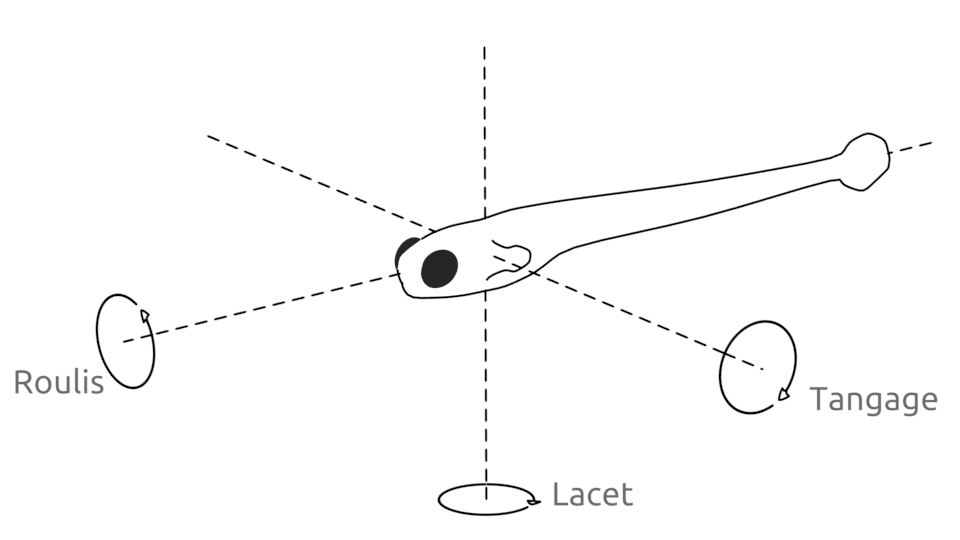
\includegraphics[width=0.8\textwidth]{./files/fish.png}
\caption{Larve de poisson zèbre dans sa position naturelle. Cette position est hors équilibre, un poisson inactif tourne sur l'axe de roulis et de tangage.}
\end{figure}

\subsection{Roulis}
Dans l'axe de roulis, la larve contrôle son équilibre par des déflexions de la queue. Si elle penche trop à gauche, elle bascule sa queue vers la droite, un peu comme un humain utiliserait ses bras pour s'équilibrer. Le contrôle postural en roulis se fait donc par une boucle de rétroaction sensorimotrice continue. L'angle de référence est de 0°, l'organe vestibulaire mesure l'écart à cet angle, et la queue le compense par une déflexion opposée. Ce comportement a été observé par Favre-Bulle \emph{et al} en simulant une rotation via une manipulation de l'utricule dans l'oreille interne par des pinces optiques. Cette étude a été réalisée en boucle ouverte, c'est-à-dire sans rétroaction, ce qui fait que la larve ne pouvait pas constater les effets de son mouvement. Une expérience de réalité virtuelle en rétroaction pourrait simuler un déséquilibre proportionnel à l'angle de la queue, ce qui permettrait à la larve d'en corriger l'angle en temps réel.

\subsection{Tangage}
Dans l'axe de tangage, la situation est plus compliquée. L'angle que fait la larve avec l'horizontale dépend de sa direction de déplacement. Par exemple, une larve se place à un angle positif lorsqu'elle nage vers le haut pour remonter à la surface et un angle négatif quand elle nage vers le bas \cite{ehrlich_primal_2019}. Cet angle constitue une référence autour de laquelle la larve cherche à se stabiliser. Ehrlich et Schoppik ont montré que le contrôle de l'angle se faisait exactement pendant les mouvements de nage \cite{ehrlich_control_2017}. La larve de poisson zèbre nage de manière discrète via des mouvements réguliers à une fréquence d'environ un par seconde en nage libre. Entre deux mouvements, elle est soumise à son déséquilibre et son nez tombe à une vitesse déterminée par sa morphologie. Lors d'un mouvement, en fonction de la force et la position des nageoires, l'angle augmente d'un coup. De plus, les auteurs suggèrent que l'initiation du mouvement est induite par l'angle ressenti. Ils ont augmenté artificiellement le déséquilibre de la larve, conduisant à une chute plus rapide. Ils ont constaté que la larve compensait ce déséquilibre supplémentaire par une augmentation de la fréquence des mouvements de nage.
Le contrôle postural en tangage est donc le résultat d'une boucle de rétroaction sensorimotrice discrète. L'angle de référence varie entre -15° et +20° environ et dépend de la direction souhaitée par le poisson. L'action de contrôle de l'angle implique à la fois la queue et les nageoires et se fait au moment des événements de nage, dont la fréquence peut être ajustée en fonction du déséquilibre.

\begin{figure}
\centering
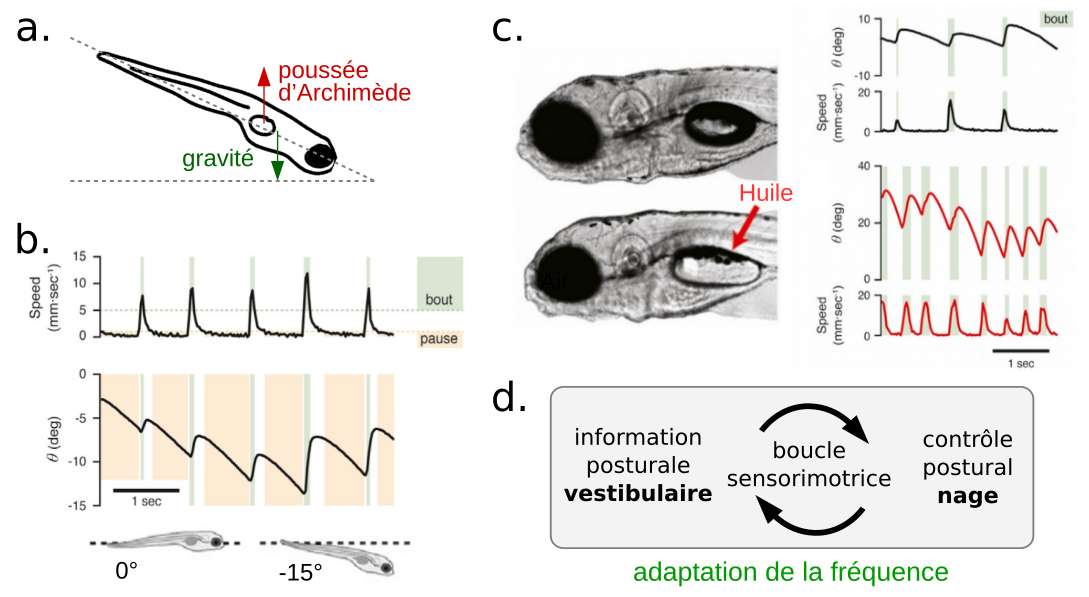
\includegraphics[width=0.9\textwidth]{./files/schoppik_movement-initiation.svg.png}
\caption{Adapté de Ehrlich et al \cite{ehrlich_control_2017}
\\
a. Le centre de gravité et de flottaison de la larve sont décalés, ce qui cause un déséquilibre dans l'axe de tangage.
\\
b. La larve nage de manière discrète (non continue), à une fréquence de ~1 Hz. Entre deux événements, la larve inactive est entraînée par son déséquilibre, nez vers le bas à une vitesse de ~6°/sec. Lors des événements de nage (pic de vitesse), l'angle est corrigé de ~6°.
\\
c. En remplaçant l'eau de la vessie natatoire par de l'huile, ce qui augmente le déséquilibre, les auteurs ont constaté une augmentation de la fréquence (diminution de l'IEI, intervalle inter-événement), ce qu'ils attribuent au contrôle de la posture via l'information vestibulaire.
\\
d. La boucle sensorimotrice discrète responsable du contrôle postural est capable d'une adaptation en fréquence suite à une perturbation de l'équilibre du poisson.}
\end{figure}

On voit ici deux boucles sensorimotrices différentes impliquée dans le contrôle postural. Ces boucles de rétroaction ont des caractéristiques différentes en termes de valeur cible et de mécanisme de contrôle. Je décris par la suite une plateforme expérimentale que j'ai mise au point afin d'étudier le contrôle postural en réalité virtuelle.

\section{Étude comportementale du contrôle postural}

\subsection{Plateforme expérimentale}

Pour reproduire la boucle de rétroaction du contrôle postural, il faut soumettre le poisson à une stimulation vestibulaire, détecter ses mouvements de queue et rétroagir sur son orientation. J'ai développé une plateforme expérimentale pour répondre à cette problématique. Elle est constituée d'une cuve où l'on place la larve, d'un système d'imagerie pour suivre les mouvements de queue, d'un projecteur pour projeter un environnement visuel sur les parois de la cuve, d'un moteur pour entraîner la plateforme sur laquelle repose le tout, et d'un ordinateur pour réaliser la boucle de rétroaction. Je décris ci-dessous les différents éléments.

\begin{figure}
\centering
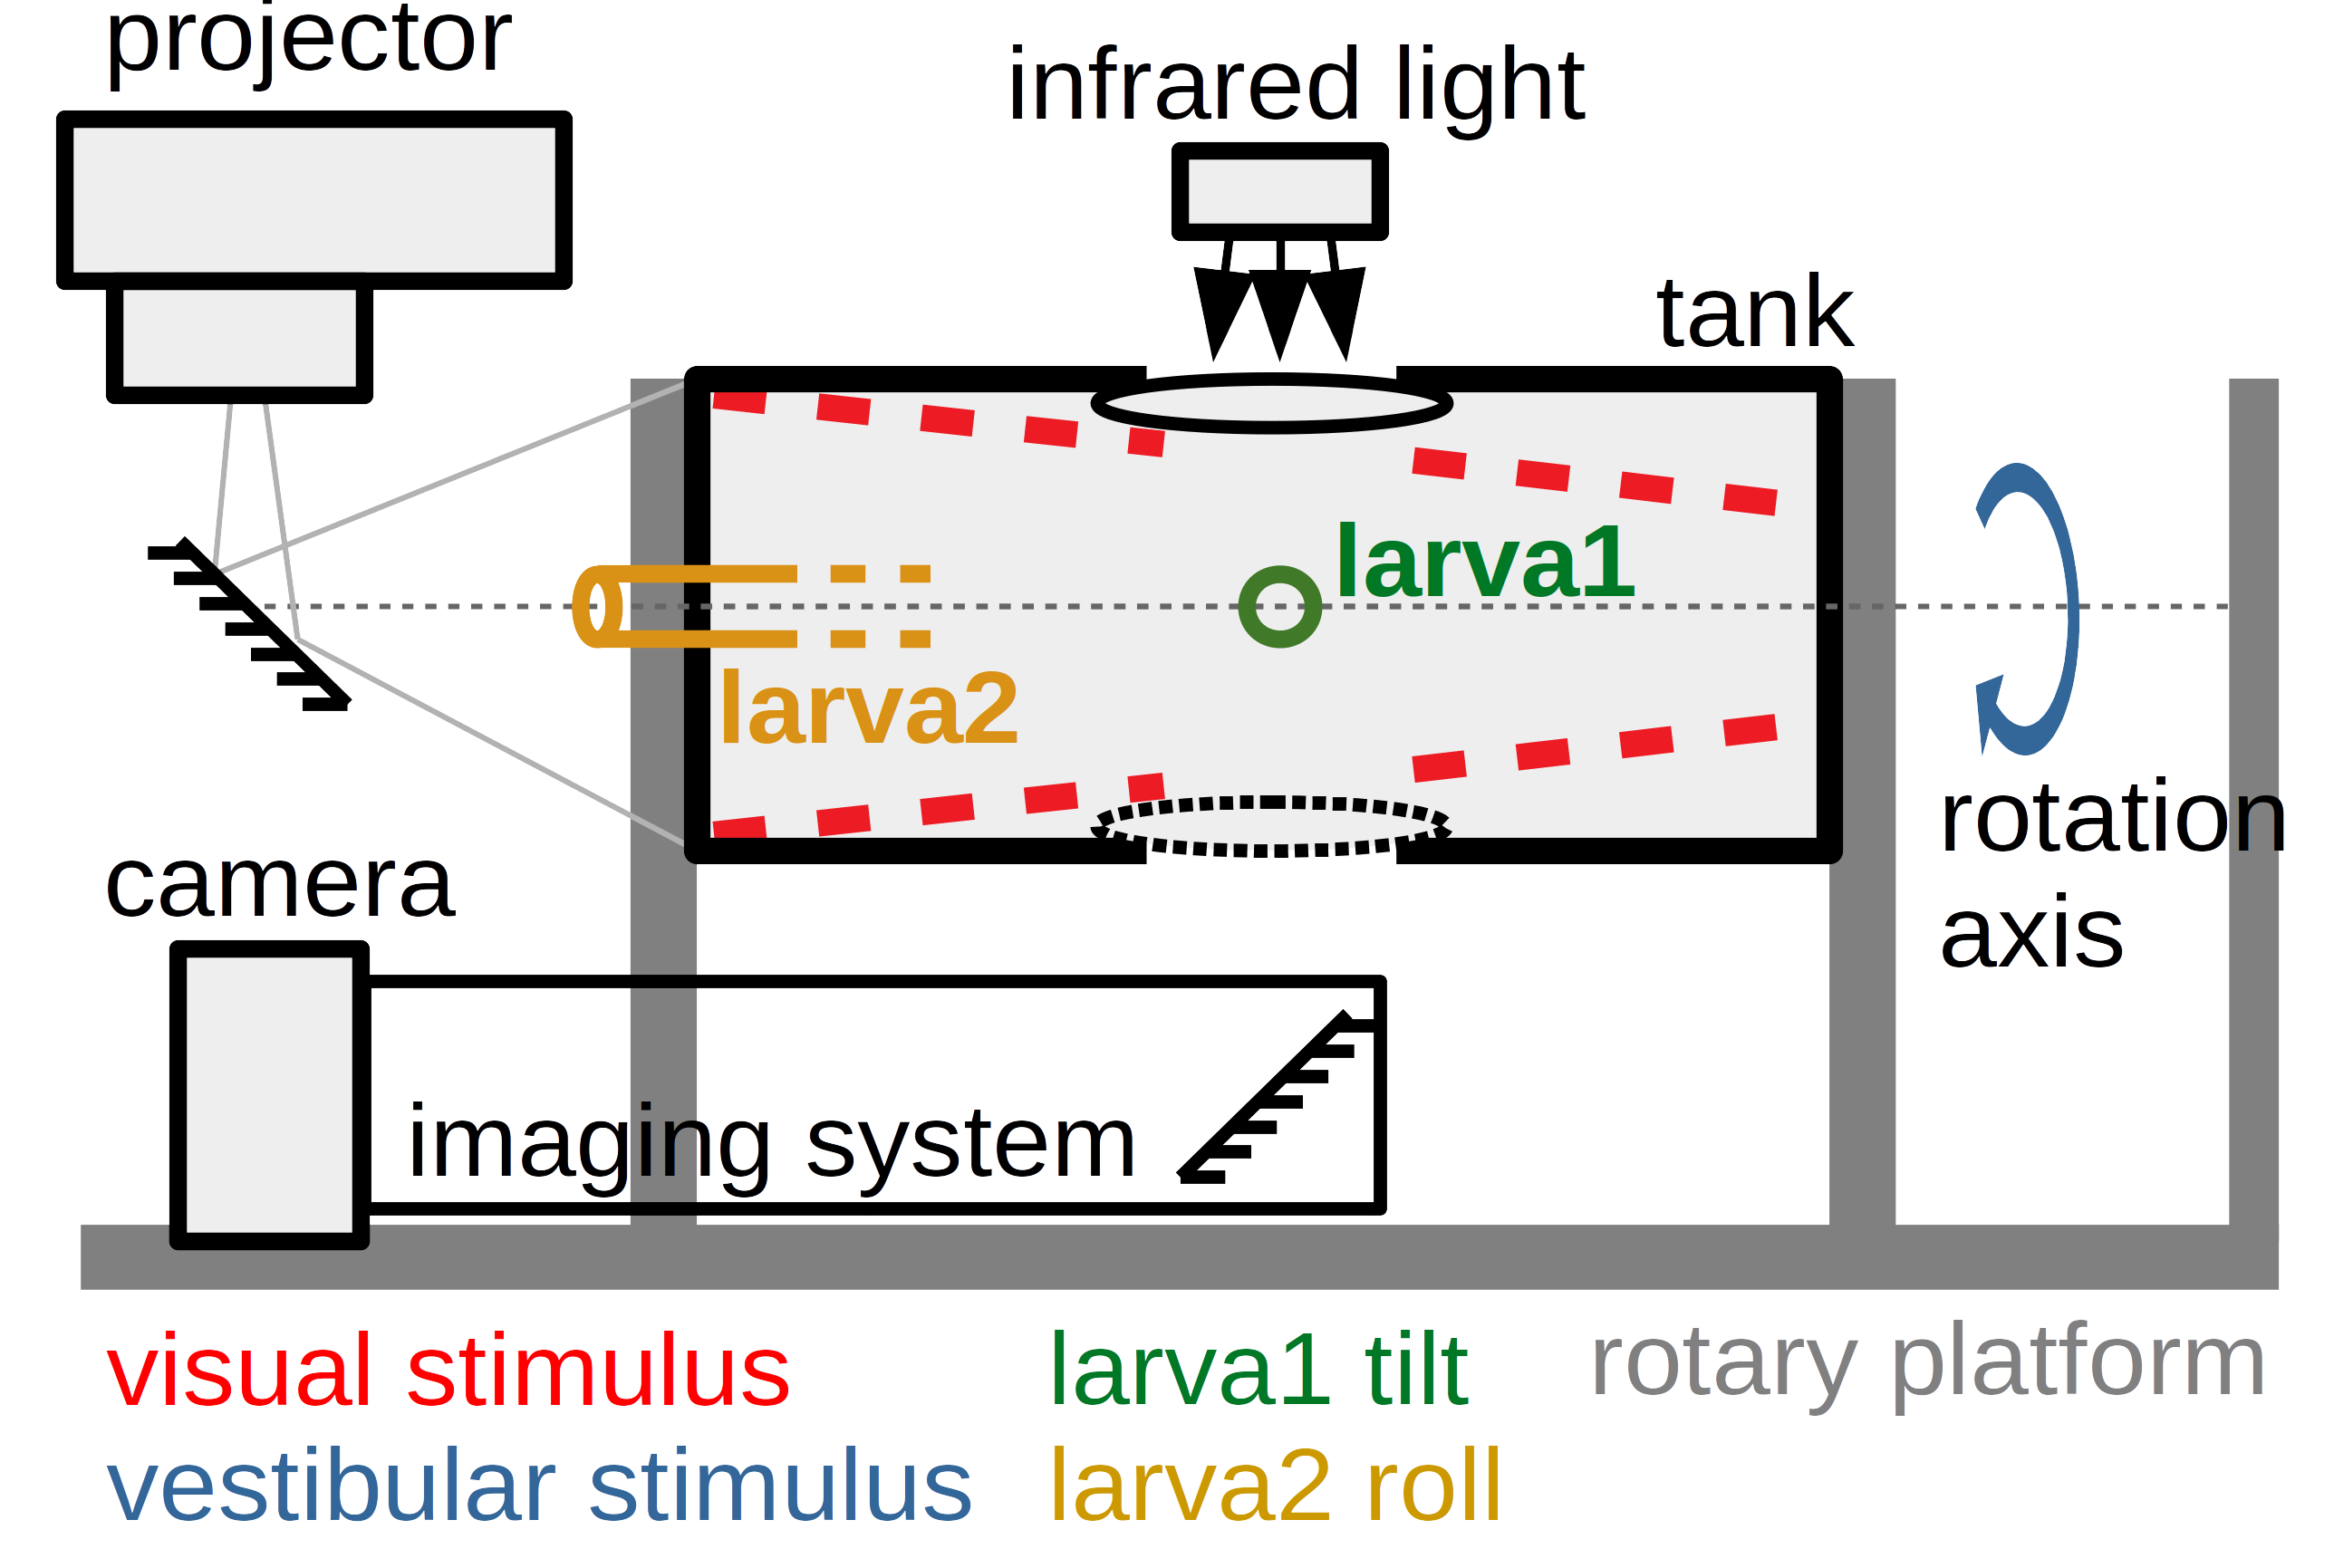
\includegraphics[width=0.7\textwidth]{./files/schema_manip.png}
\caption{Plateforme expérimentale permettant d'étudier le contrôle postural d'une larve de poisson zèbre pendant une boucle de rétroaction.}
\end{figure}

\subsubsection{Stimulation vestibulaire}
Le but de la cuve rotative est de soumettre le poisson à un stimulus vestibulaire contrôlé, et de pouvoir agir rapidement sur la commande (position angulaire, vitesse angulaire). Le moteur que j'ai utilisé pour entraîner la plateforme est le modèle DMAC17 de l'entreprise [midi-ingéniérie](http://www.midi-ingenierie.com/). Le modèle était assez ancien et ne disposait que d'une interface rudimentaire, j'ai donc dû réimplémenter une commande série pour communiquer avec le microcontrôleur de la commande moteur. Finalement, la communication introduit une latence de quelques dizaines de millisecondes et impose un délai entre deux instructions. Cela semble cependant suffisant pour garantir une bonne impression de réalité virtuelle, puisque chez l'humain, les effets liés à la latence commencent à se faire sentir à partir de 75 ms \cite{waltemate_impact_2016}. Un problème que j'ai rencontré au début était les mouvements de l'eau dans la cuve. Le poisson y est très sensible via sa ligne latérale postérieure, ce qui faussait les expériences. En modifiant légèrement la cuve, j'ai pu maintenir l'eau de la cuve pratiquement immobile.

\subsubsection{Imagerie et analyse}
Pour détecter de manière fiable les mouvements de queue du poisson, j'ai mis au point un système d'imagerie adapté. Le système doit être léger et compact, afin de limiter le couple lors de la rotation de la plateforme et être insensible aux vibrations. Le poisson est éclairé par une lampe infrarouge à travers un diffuseur et une fenêtre située en haut de la cuve. En bas de la cuve, une autre fenêtre étanche laisse passer la lumière vers un miroir sur lequel pointe une caméra équipée d'un objectif grossissant et d'un filtre infrarouge. L'utilisation de la lumière infrarouge, invisible pour le poisson, permet de conserver la même qualité d'image quel que soit l'environnement visible pour le poisson. Les fenêtres sont les plus petites possible et situées dans l'extrémité du champ de vision du poisson afin de contrôler au mieux son environnement visuel. Le miroir permet de conserver la caméra et l'objectif proche de l'axe de rotation de la plateforme, pour limiter le bras de levier.
L'objectif du système d'imagerie est choisi pour que le poisson soit imagé sur un nombre réduit de pixels de la caméra. Ainsi, le transfert de donnée depuis la caméra vers l'ordinateur et le traitement de l'image sont rapides, ce qui permet de ne pas ralentir la rétroaction. Le traitement de l'image est simpliste mais fonctionnel. Il consiste à appliquer les fonctions suivantes :

- filtre de Sobel (fonction `edge` de Matlab, option `sobel`)
- dilatation (fonction `imdilate`)
- remplissage (fonction `imfill`)
- ouverture (fonction `bwareaopen`)
- ellipse équivalente (fonction `regionprops`, option `Orientation` )

Ce qui permet de trouver l'angle du poisson de manière reproductible d'une image sur l'autre, afin de détecter les mouvements de queue.

\begin{figure}
\centering
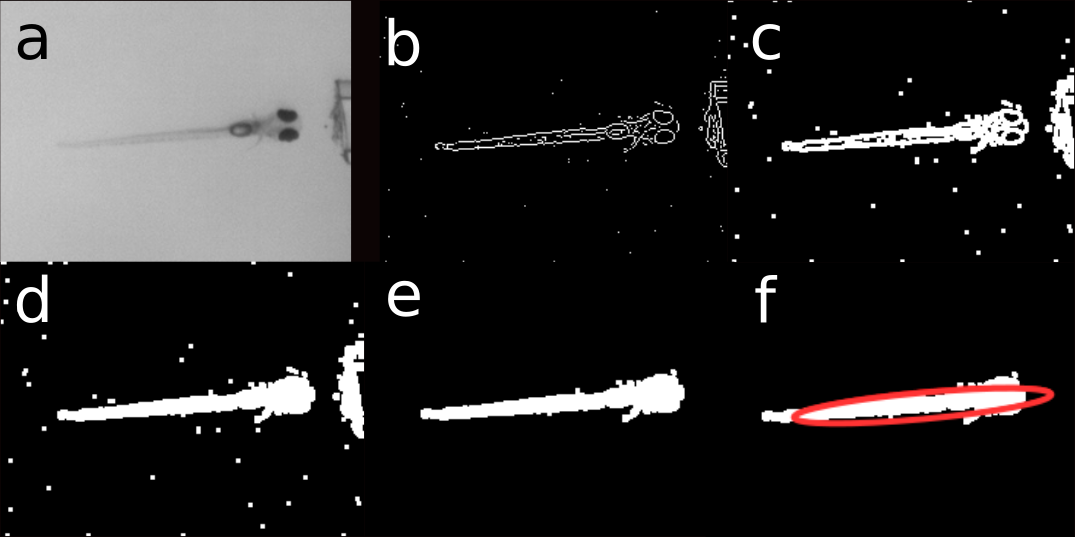
\includegraphics[width=0.8\textwidth]{./files/image_process.png}
\caption{Traitement d'image en cinq étapes pour obtenir l'angle du poisson. a) image originale sous éclairage infrarouge b) filtre de Sobel c) dilatation morphologique d) remplissage des contours e) ouverture morphologique f) ellipse équivalente via les moments d'ordre deux de l'image}
\end{figure}

% TODO Volker add figure with tail bend / struggle

\subsubsection{Stimulation visuelle}
Pour avoir un contrôle très souple sur l'environnement visuel du poisson du point de vue des couleurs, de la luminosité, et des formes, la solution idéale est un projecteur. Afin d'obtenir un bon contraste, les parois de la cuve sont coniques et blanches, réalisées dans un cylindre de PVC. Un cache évite d'éclairer directement le poisson pour ne pas perturber son environnement visuel. Les motifs sont réalisés à l'aide de \href{http://psychtoolbox.org/}{psychtoolbox}, une bibliothèque conçue pour l'affichage de stimulations visuelles. Pour conserver une fréquence d'affichage indépendant de la boucle de rétroaction et ainsi garantir un taux constant d'images par seconde d'expérience en expérience, j'ai séparé le processus de la boucle principale, avec laquelle il communique par le protocole TCP/IP.

\subsubsection{Insertion de la larve}
Pour immobiliser la larve de poisson zèbre, il est fréquent de la piéger dans un gel d'agarose à basse température de fusion concentré à 2\% aspiré par un capillaire en verre de diamètre intérieur 0.8 mm. La larve peut ainsi être insérée et maintenue par des trous de 1.4 mm, le diamètre extérieur du capillaire. Il en existe deux dans ma cuve : l'un sur l'axe de rotation pour étudier la réponse comportementale à une stimulation en roulis, l'autre perpendiculaire pour étudier la réponse à une stimulation en tangage. Afin d'observer les mouvements de la queue, je la libère en retirant la partie du boudin d'agarose qui l'entoure. 

\begin{figure}
\centering
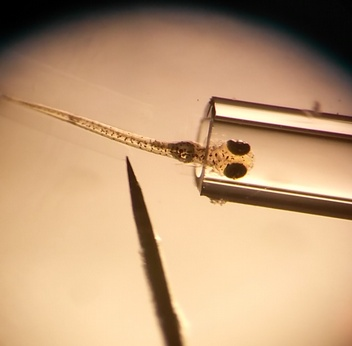
\includegraphics[width=0.6\textwidth]{./files/prepa_larve.png}
\caption{À l'aide d'un scalpel, un boudin d'agar est retiré de la queue d'une larve pour lui permettre de bouger. La larve est retenue par la tête et le corps, l'autre partie du boudin étant tenue par le capillaire en verre. }
\end{figure}

\subsection{Protocoles et résultats}

\subsubsection{Test par l'OMR}
Après avoir inséré un poisson dans la cuve, je le laisse reposer une à deux minutes pour lui permettre de s'adapter à son nouvel environnement. Je teste ensuite son réflexe optomoteur (OMR). Si le poisson ne réagit pas à cette stimulation visuelle, il est possible que sa vision ou sa motricité ne fonctionne pas, ou que son cerveau ne soit pas dans un état propice à l'étude de son système sensori-moteur. Pour tester l'OMR, je présente une alternance de bandes noires et blanches d'une taille apparente de trente degrés défilant à une vitesse apparente de vingt degrés par seconde, uniquement sur la partie basse de l'environnement visuel. Ce protocole est inspiré par celui présenté par Kris Severi \cite{severi_neural_2014}. J'ai réalisé ce test en boucle ouverte, c'est-à-dire sans rétroaction. Dans ce régime, le poisson présente un phénomène d'habituation si la stimulation dure trop longtemps, j'ai donc alterné des périodes de dix secondes de bandes fixes et dix secondes de bandes mobiles.

% This is the protocol also in the literature. If I remember correctly this is what Kris used in here paper. It would be good if you add references here

\begin{figure}
\centering
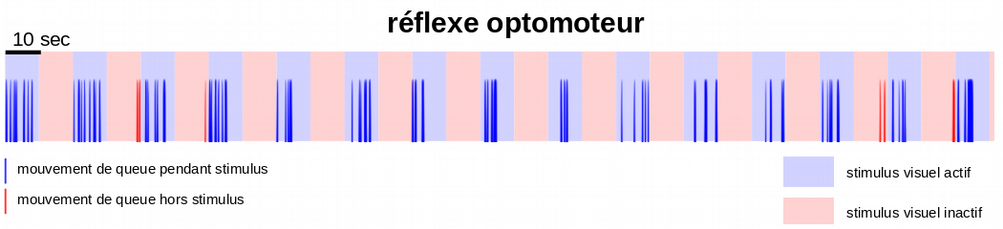
\includegraphics[width=0.9\textwidth]{./files/omr.png}
\caption{Expérience d'OMR en boucle ouverte. On voit que le poisson nage systématiquement en présence de stimulation visuelle (440 événements sur 150 secondes) et qu'il nage très rarement en absence de stimulation visuelle (22 événements sur 150 secondes).}
\label{FigOMRopenloop}
\end{figure}

Ces expériences sur le réflexe optomoteur montrent que le stimulus visuel projeté est suffisant pour étudier les réponses de la larve à son environnement visuel (Fig. \ref{FigOMRopenloop}).

\subsubsection{Rétroaction vestibulaire}
Pour mettre en place la boucle de rétroaction vestibulaire, je me suis inspiré de l'étude en nage libre de Ehrlich \emph{et al} \cite{ehrlich_control_2017}. J'ai choisi une vitesse de chute de 6°/s et une correction angulaire rapide de 10° lors d'un mouvement (en 100 ms environ). Ainsi, le poisson peut se maintenir à un angle fixe avec un mouvement toutes les 1.6 secondes. Si le poisson est immobile, son angle diminue jusqu'à l'angle limite que j'ai fixé à -60°. Ces expériences ont été réalisées dans le noir ou en éclairage uniforme, pour étudier la perception vestibulaire indépendamment de la perception visuelle.

\begin{figure}
\centering
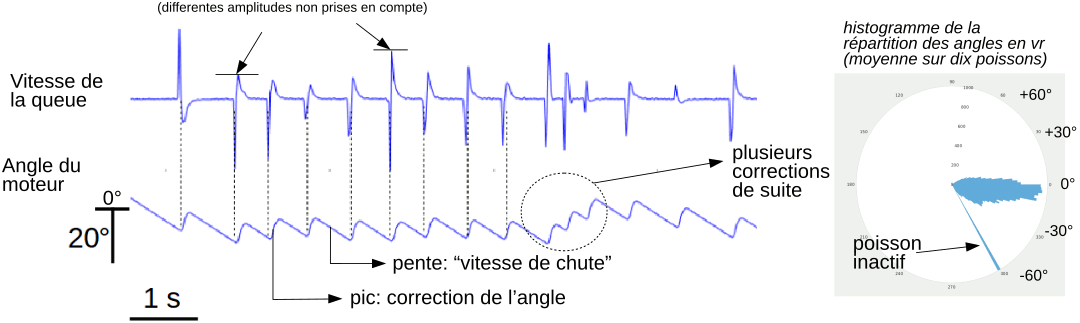
\includegraphics[width=0.9\textwidth]{./files/vestibular_feedback.svg.png}
\caption{Zoom sur un exemple de contrôle de posture dans une boucle de rétroaction virtuelle. Le poisson est soumis à un stimulus vestibulaire constant (pente constante) en l'absence de comportement. Lors d'un mouvement de nage, une rétroaction sur l'angle de la plateforme simule une correction d'angle du poisson.}
\end{figure}

Les paramètres de la boucle sont la vitesse de chute et l'angle de correction lors du mouvement. Pour répondre à une modification de ces paramètres, le poisson doit adapter la fréquence de ses mouvements, car l'amplitude n'est pas prise en compte. Ainsi, à correction angulaire fixe, si la vitesse de chute augmente, comme dans l'expérience de la vessie natatoire remplie d'huile, le poisson doit augmenter la fréquence de ses mouvements. Au contraire, à vitesse de chute fixe, si la correction angulaire augmente, le poisson doit baisser la fréquence de ses mouvements. C'est effectivement ce que l'on constate dans les expériences, où une vitesse de chute de 2°/s, 4°/s et 6°/s avec une correction angulaire de 10° entraînent respectivement chez la larve une fréquence de mouvement de 0.2 Hz, 0.4 Hz, et 0.6 Hz en moyenne.

\begin{figure}
\centering
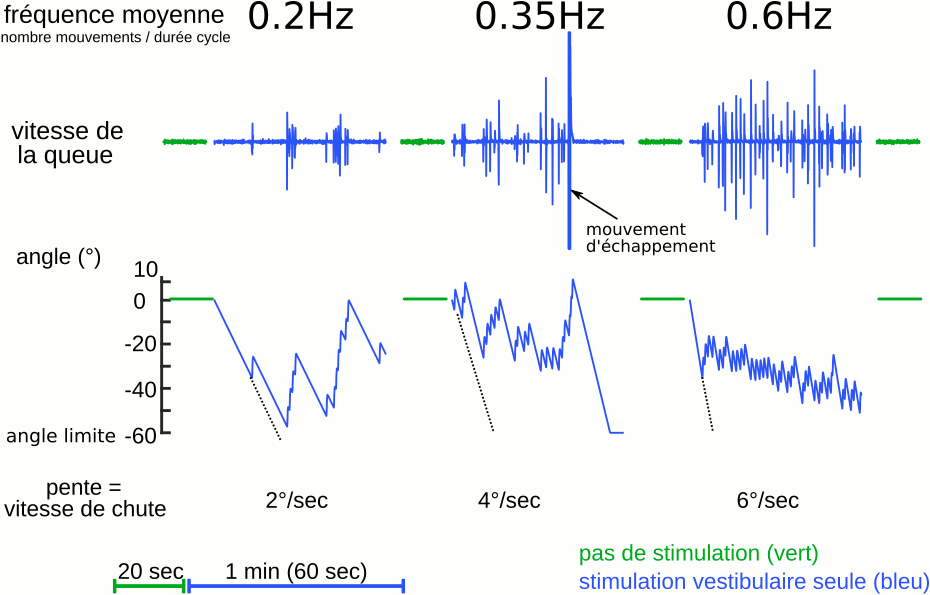
\includegraphics[width=0.8\textwidth]{./files/variation-vitesse.svg.png}
\caption{
Réponse d'une larve à une variation de la vitesse de chute. Trois cycles de une minute de stimulation vestibulaire sont séparés de pause de dix secondes. Le poisson se maintient autour d'un angle de -20° quelle que soit la vitesse de chute imposée, en adaptant la fréquence de ses mouvements.
\\
La fréquence moyenne du deuxième cycle est légèrement inférieure à sa valeur attendue (0.35 Hz au lieu de 0.4 Hz). Cela est du au fait que, suite à un mouvement d'échappement, le poisson est totalement inactif à la fin du cycle et stationne à -60°. Si l'on calcule la fréquence en ignorant les dix dernières secondes, la fréquence moyenne est bien de 0.4 Hz.
}
\end{figure}


La principale difficulté de ces expériences est le fait que le poisson peut devenir inactif et stationner à l'angle minimal autorisé par le système (-60°). C'est pour cette raison que la durée choisie pour les cycles est relativement courte (60 secondes). À la fin d'un cycle, le poisson est ramené à l'angle de référence (0°). Cela évite que le poisson reste trop longtemps inactif, état dans lequel il est impossible d'étudier le contrôle postural. Pour obtenir des fréquences représentatives, il faut donc les calculer uniquement sur les périodes d'activité.

On observe ce même comportement sur des larves dans une boîte de pétri : de temps en temps elles cessent toute activité et reposent sur le fond de la boîte. La boucle de rétroaction du contrôle postural est alors en pause. Dans le cas d'une larve prisonnière d'un boudin d'agarose, les périodes d'inactivité font souvent suite à un mouvement d'échappement (\emph{struggle}), pendant lequel la larve tente de s'échapper en se tortillant sur elle-même avec des mouvements de très grande amplitude.

\subsubsection{Protocole multimodal}
L'intérêt de l'environnement virtuel est qu'il est possible de contrôler à la fois la stimulation vestibulaire et la stimulation visuelle. Après avoir étudié le contrôle postural dans le noir, j'y ai ajouté une composante visuelle. L'objectif est de comparer la réponse en cas de stimulation multimodale par rapport aux réponses en présence des deux stimuli séparément.

\begin{figure}
\centering
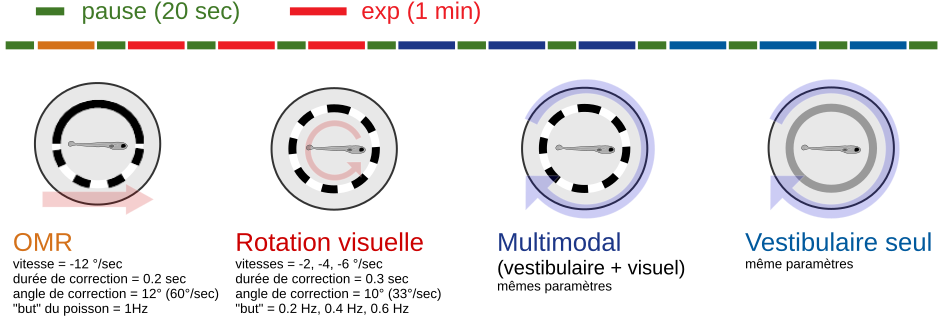
\includegraphics[width=0.9\textwidth]{./files/protocole_multimodal.svg.png}
\caption{
Exemple de protocole multimodal, faisant intervenir à la fois une stimulation vestibulaire et une stimulation visuelle. Des cycles d'une minute sont séparés par des pauses de vingt secondes.
}
\end{figure}

Le protocole commence par un cycle d'OMR qui permet d'évaluer le niveau d'activité du poisson. S'il ne répond pas à cette stimulation, l'expérience est interrompue pour passer au poisson suivant, ce qui évite d'observer pendant un quart d'heure une larve immobile. Ensuite vient une phase de stimulation purement visuelle avec rotation de l'ensemble de l'environnement, tout autour du poisson. Pendant cette phase, l'information visuelle indique au poisson qu'il tourne, ce qui est en conflit avec l'information vestibulaire. La partie inférieure du champ visuel est similaire à une stimulation d'OMR, mais la partie supérieure diffère. Il est de toute façon difficile de différencier les deux. Ensuite, en conservant le motif de la phase visuelle en position fixe dans le référentiel du laboratoire, la cuve tourne avec le poisson pour stimuler le système vestibulaire, utile au contrôle postural. Pendant cette phase, les deux modalités sensorielles sont cohérentes. Elles indiquent toutes les deux au poisson qu'il est en train de tourner. Ensuite, le motif est remplacé par un éclairage uniforme d'intensité moyenne identique. Cela permet de conserver une luminosité ambiante dans la cuve identique au cycle précédent. Cette phase est celle exposée précédemment, dans la partie sur la rétroaction vestibulaire. Chaque phase est séparée en trois sous-phases, avec trois vitesses de stimulus différentes (2, 4, et 6 degrés par seconde), pour étudier l'adaptation aux conditions virtuelles.

\begin{figure}
\centering
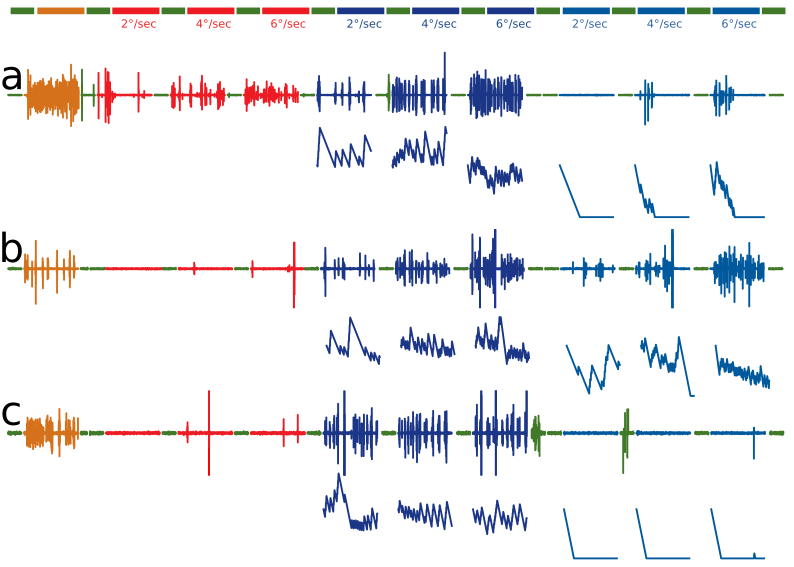
\includegraphics[width=0.8\textwidth]{./files/raw_data.svg.png}
\caption{
On voit ici le protocole appliqué sur trois poissons différents. Dans tous les cas, la réponse optomotrice fonctionne, mais on voit des différences au niveau des autres stimuli. Le poisson (a.) répond bien à la stimulation visuelle, mais quasiment pas à la stimulation vestibulaire, le poisson (b.), au contraire, ne répond pas à la stimulation visuelle (bien qu'il réponde à l'OMR), mais répond à la stimulation vestibulaire pure. Le poisson (c.) ne répond ni à la stimulation visuelle pure, ni à la stimulation visuelle pure, mais répond comme les deux autres pendant le cycle multimodal.
\\
Ces comportements spécifiques à un poisson sont reproductibles. Le protocole a été répété cinq fois sur le poisson (a.) avec toujours la même réponse.
}
\end{figure}

La réponse des larves à ce protocole est très variable. De nombreuses données sont inutilisables à cause d'une larve immobile après un mouvement d'échappement, mais dans les données restantes, certains poissons montrent une bonne réponse principalement au stimulus vestibulaire seul, d'autres au stimulus visuel seul, alors que la plupart répondent bien pendant le cycle multimodal. Il semble donc qu'en fonction des poissons l'importance relative des différentes modalités sensorielles dans le contrôle postural soit variable. Pour certains poissons, cependant, la présence simultanée des deux modalités sensorielles semble nécessaire au contrôle postural. Cela peut être interprété de la manière suivante.

Pendant les phases unimodales visuelles, les sensations visuelle et vestibulaire sont en conflit, ce qui peut réduire et même supprimer la réponse motrice, la force de cet effet variant d'un poisson à l'autre. Dans les phases unimodales vestibulaires, le poisson ne reçoit aucune information visuelle sur sa position et la réponse comportementale peut être affaiblie par un manque de fiabilité de l'information vestibulaire. Au contraire, pendant les phases de stimulus multimodal cohérent, on remarque une réponse comportementale forte, augmentée par l'intégration multisensorielle.

% During the unimodal visual phases the visual and vestibular sensations are in conflict reducing or suppressing the motor response. The strength of this effect varies between fish. In the unimodal vestibular case where the fish does not receive and visual information about its body rotation the behavioral response might be weak due to the unrelieability of the vestibular stimulus. However, in the coherent multimodal case we see a strong multisensory enhanced behaviorial response 

\subsubsection{Interprétation}
Malgré ces comportements individuels variables, on peut analyser globalement la réponse des larves. La métrique utilisée est la fréquence moyenne des mouvements, calculée comme le rapport entre la quantité de mouvements de nage et la durée du cycle. Cette métrique inclut les périodes d'inactivité qui suivent un mouvement d'échappement, ce qui fausse légèrement la valeur, comme montré dans l'exemple de rétroaction vestibulaire. On observe néanmoins deux phénomènes : le poisson est capable de moduler son activité en fonction de la force du stimulus, et le poisson a une réponse plus forte en présence de deux stimuli cohérents .

\begin{figure}
\centering
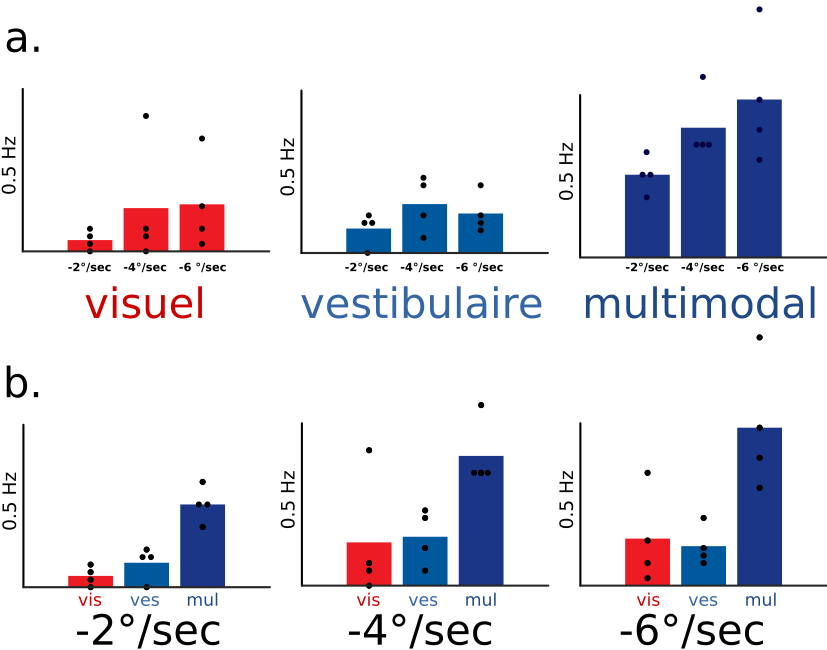
\includegraphics[width=0.8\textwidth]{./files/stats.svg.png}
\caption{
Analyse réalisée sur dix poissons différents parmi trente soumis au protocole. Les valeurs à zéro (poisson entièrement inactif) sont retirées, et il reste donc environ quatre points par moyenne.
\\
a. Pour chaque cycle, on observe une adaptation du poisson à la force du stimulus. Le poisson est capable d'adapter sa fréquence de nage pour se stabiliser par rapport à une information visuelle ou vestibulaire.
\\
b. Pour chaque vitesse de stimulus, on observe une réponse moyenne différente en fonction du type de stimulus. Alors que le stimulus vestibulaire et visuel pur sont d'efficacité comparable, la présence simultanée des deux modalités sensorielles entraîne globalement une meilleure réponse chez les larves.
}
\end{figure}

% TODO Volker Perspective and interpretation of the results is still to develop. 

On a montré qu'il était possible de reproduire la boucle de rétroaction sensorimotrice du contrôle postural dans un environnement virtuel. Une des principales limitations est l'immobilisation de la larve, qui provoque des mouvements violents d'échappement suite auxquels la larve est inactive pendant une longue durée. Cela réduit considérablement la quantité de données exploitables (environ 90\% des expériences sont en partie ou totalement inutilisables), les données présentées ici sont donc statistiquement faibles.

Ces résultats montrent qu'un réflexe \emph{a priori} vestibulaire comme le contrôle postural est en réalité largement altéré par d'autres modalités sensorielles comme le système visuel. On peut supposer que la sensation tactile, qui permet au poisson de sentir les écoulements de fluide, joue également un rôle (que je n'ai pas testé). La reproduction de la boucle sensorimotrice dans un environnement en réalité virtuelle ouvre la possibilité d'étudier les mécanismes cérébraux qui en sont à l'origine. Pour comprendre en profondeur ces mécanismes, il est nécessaire de simuler un environnement sensoriel riche  

Une piste d'évolution importante serait de limiter ces comportements d'échappement. 
% escape/startle/struggle
%TODOcite
% - Glia Accumulate Evidence that Actions Are Futile and Suppress Unsuccessful Behavior
% - Escape Behavior Elicited by Single, Channelrhodopsin-2-Evoked Spikes in Zebrafish Somatosensory Neurons
% - Imaging the Functional Organization of Zebrafish Hindbrain Segments during Escape Behaviors
% - Evidence for a Widespread Brain Stem Escape Network in Larval Zebrafish
% - Imaging escape and avoidance behavior in zebrafish larvae
Ceux-ci diminuent largement l'échantillon statistique en inhibant l'activité du poisson pendant de longues périodes, ce qui rend l'analyse difficile. Cette amélioration pourrait être obtenue en modifiant la manière dont le poisson est retenu immobile et en ajustant les paramètres de rétroaction en fonction des poissons. 

\subsection{Conclusion}

% TODO Volker Perspective and interpretation of the results is still to develop. 